\documentclass[a4paper,12pt]{article}
\usepackage{graphicx}
\usepackage{listings}
\usepackage{xcolor}
\usepackage{hyperref} 
\usepackage{caption} 
\usepackage{subcaption}
\usepackage{fancyhdr} 
\usepackage{geometry}
\usepackage{titling}
\usepackage{tocbibind}
\usepackage{float} 
\usepackage{array}
\usepackage{longtable}
\usepackage[dvipsnames]{xcolor}

\lstset{
    language=C++,
    basicstyle=\ttfamily\small,
    keywordstyle=\color{blue}\bfseries,
    commentstyle=\color{green!60!black},
    stringstyle=\color{red},
    numbers=left,
    numberstyle=\tiny\color{gray},
    stepnumber=1,
    showstringspaces=false,
    tabsize=4,
    breaklines=true,
    breakatwhitespace=true
}

\lstset{
    classoffset=1,
    morekeywords={class, struct, typename}, 
    keywordstyle=\color{teal}\bfseries,
    classoffset=2,
    morekeywords={int, float, double, bool, char, long, short, \$},
    keywordstyle=\color{cyan},
    classoffset=3, 
    morekeywords={MessageBox, string, Move, Game, Stack, Queue, UI, Game, Board, Block, Player, List},
    keywordstyle=\color{ForestGreen}\bfseries,
    classoffset=4,
    morekeywords={ Push, Pop, Enqueue, Flip, Dequeue,Add,Remove,GetSize,Size,GetBlock, GetBoard, GetRank, GetFile},
    keywordstyle=\color{Tan}\bfseries, 
    classoffset=0 
}


\geometry{top=3cm, bottom=3cm, left=2.5cm, right=2.5cm}

\begin{document}
\thispagestyle{empty} 

\vspace*{1cm} 

\begin{center}
    {\Huge\textbf {Chess Project}}  
    \vspace{1cm}  

    \begin{figure}[h!]
        \centering
        
\includegraphics[width=0.3\textwidth]{Images/logo.jpg}
    \end{figure}
    
    {\large Session 2023-2027}\\[0.2cm]
    \vspace{0.7cm}
    {\Large\textbf {Submitted By: }}\\[0.6cm]
    {\large {Mohammad Bilal \space\space\space 2023-CS-168}}\\[0.6cm]
    {\Large\textbf {Supervised By: }}\\[0.6cm]
    {\large {Mr. Nazeef Ul Haq }}\\[0.4cm]
    {\large {Mr. Waseem }}\\[0.6cm]
    {\Large\textbf {Course: } CSC-200L}\\[1.2cm]
    {\LARGE \textbf{ Department of Computer Science}}\\[0.7cm]
    {\Huge \textbf{University of Engineering and}}\\[0.5cm]
    {\Huge \textbf{Technology, Lahore}}\\[0.5cm]
    \vfill
\end{center}

\thispagestyle{empty} 

% all the contents table, figures and tables must have no text on heder footer 

\renewcommand{\contentsname}{Table of Contents}

\tableofcontents

\newpage

\pagestyle{fancy}
\fancyhf{}
\fancyhead[L]{\textbf{Chess Project}}
\fancyfoot[R]{{\thepage}}
\fancyfoot[L]{{MOHAMMAD BILAL}}

\section{Project Overview}

\subsection{Description}
This project is a Chess Game developed using the WPF framework in C\#. It leverages the .NET Framework version v4.8 and provides an engaging platform for both multiplayer and single-player modes. The single-player mode offers three difficulty levels: easy, medium, and hard. Additionally, the game adheres strictly to FIDE rules, includes time controls (1m, 3m, 5m, and 10m), and supports advanced features like Undo functionality, offering a draw, and move validation. 

\subsection{Motivation}
The motivation for creating this project stemmed from two key factors:
\begin{itemize}
    \item A desire to learn and understand the practical use of data structures in building software applications.
    \item A personal admiration for the game of Chess and an eagerness to develop my own version of it with modern features and functionalities.
\end{itemize}

\subsection{Objectives}
The objectives of the project include the following.
\begin{itemize}
    \item Design and implement a chess game that adheres to the FIDE rules.
    \item To integrate both multiplayer and Player vs. Computer modes with varying difficulty levels.
    \item Demonstrate the use of data structures such as arrays, lists, linked lists, stacks, and graphs in a real-world project.
    \item To enhance understanding of WPF and the.NET framework.
\end{itemize}

\subsection{Target Audience}
This project aims to:
\begin{itemize}
    \item Beginners and intermediate programmers who wish to explore the practical application of data structures.
    \item Developers interested in creating games using WPF and the.NET Framework.
\end{itemize}

\subsection{Features}
\begin{longtable}{|p{0.25\textwidth}|p{0.7\textwidth}|}
    \caption{Game Features}
    \hline
    \textbf{Feature} & \textbf{Description} \\
    \hline
    Multiplayer Mode & Allows two human players to play against each other. \\
    \hline
    Notation & Proper Display of Moves Notation for ease of users. \\
    \hline
    Player vs. Computer Mode & Enables a single player to compete against the AI with three difficulty levels: easy, medium, and hard. \\
    \hline
    Time Controls & Provides four time control options: 1 minute, 3 minutes, 5 minutes, and 10 minutes. \\
    \hline
    FIDE-Compliant Rules & Adheres to official Chess rules, including castling, en passant, and pawn promotion. \\
    \hline
    Undo Functionality & Allows players to undo their last move. \\
    \hline
    Offer Draw & Players can offer a draw during the game. \\
    \hline
    Resign & Players can resign during the game. \\
    \hline
\end{longtable}

\subsection{Operational Details}
\begin{longtable}{|p{0.25\textwidth}|p{0.7\textwidth}|}
    \caption{Technology Stack}
    \hline
    Framework & .NET Framework v4.8. \\
    \hline
    UI Framework & WPF (Windows Presentation Foundation)   \\
    \hline
    Language & C\# \\
    \hline
    IDE & Visual Studio 2022 Community Edition \\
    \hline
\end{longtable}

\section{Use Cases}

\subsection{Landing Page}

\begin{longtable}{|m{0.25\textwidth}|m{0.7\textwidth}|}
    \caption{Landing Page} \\
    \hline
    Name & Landing page \\
    \hline
    Actor & Player \\
    \hline
    Description & It displays the options that the player can explore in this game. \\ 
    \hline
    \centering UI & 
    \begin{center}
        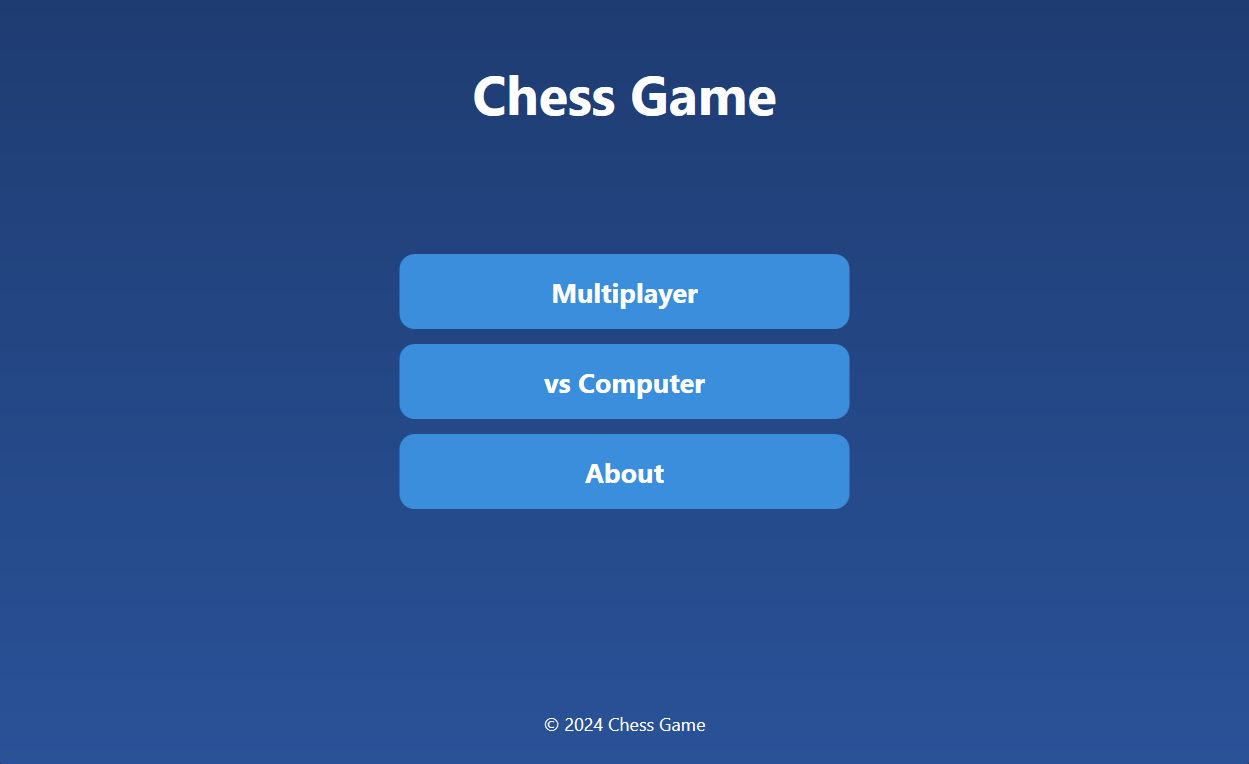
\includegraphics[height=2.7in]{Images/Use Cases/landingPage.png}
    \end{center} \\ 
    \hline
\end{longtable}

\subsection{Multi-Player Select Options}

\begin{longtable}{|m{0.25\textwidth}|m{0.7\textwidth}|}
    \caption{Multi-Player Select Options} \\
    \hline
    Name & Multi-player pop-up \\
    \hline
    Actor & Player \\
    \hline
    Description & It displays the time controls and the color that the player can select. \\ 
    \hline
    \centering UI & 
    \begin{center}
        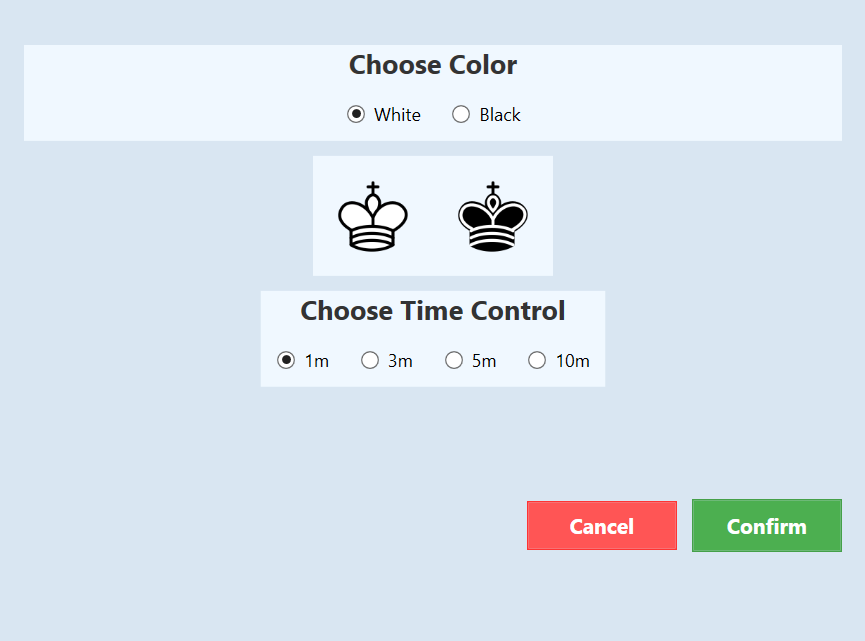
\includegraphics[height=2.7in]{Images/Use Cases/multiplayerSelectOptions.png}
    \end{center} \\ 
    \hline
\end{longtable}

\subsection{Multi-Player Page}

\begin{longtable}{|m{0.25\textwidth}|m{0.7\textwidth}|}
    \caption{Multi-player Page} \\
    \hline
    Name & Game page \\
    \hline
    Actor & Player \\
    \hline
    Description & It is the main page where the game is played. It displays the board, moves, dead pieces and the additional buttons for better experience \\ 
    \hline
    \centering UI & 
    \begin{center}
        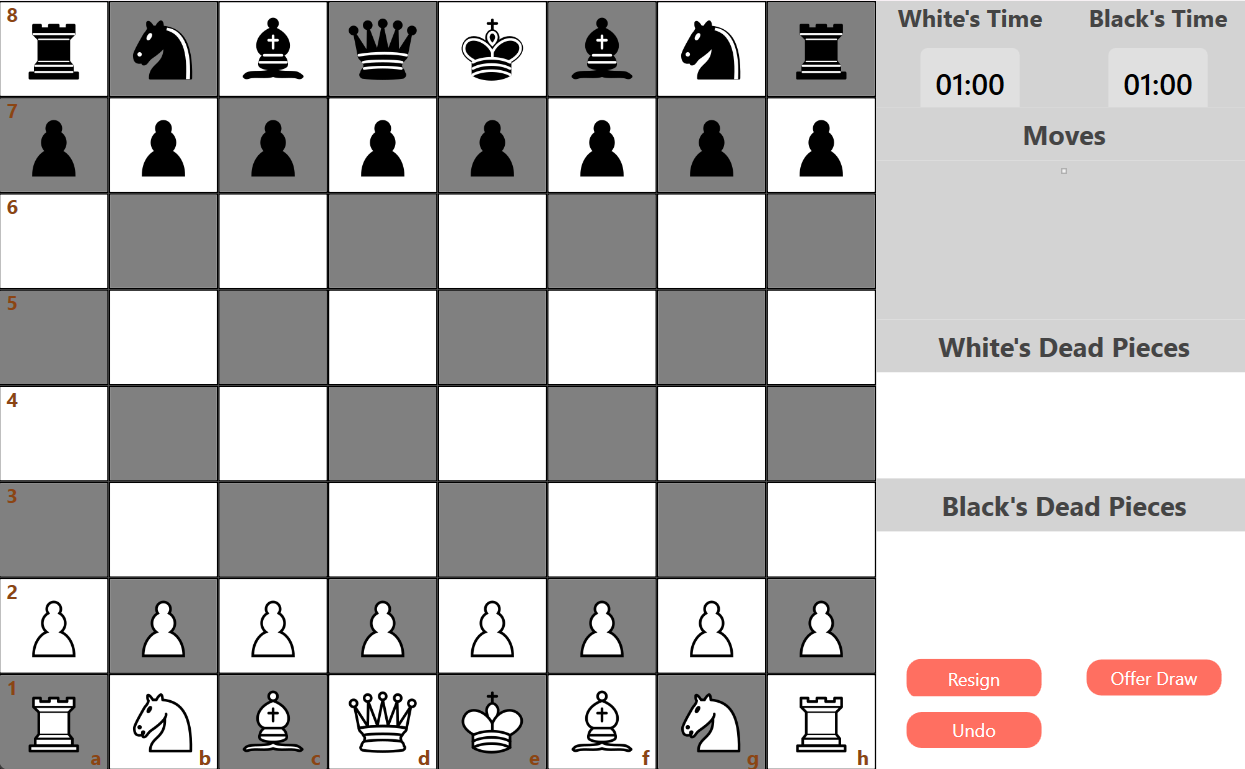
\includegraphics[height=2.7in]{Images/Use Cases/multiplayerPage.png}
    \end{center} \\ 
    \hline
\end{longtable}

\subsection{Promotion Select Options}

\begin{longtable}{|m{0.25\textwidth}|m{0.7\textwidth}|}
    \caption{Promotion Select Options} \\
    \hline
    Name & Promotion selection page \\
    \hline
    Actor & Player \\
    \hline
    Description & It displays the options (Queen, Knight, Bishop and Rook) that your pawn can promote to on reaching enemies last rank.\\ 
    \hline
    \centering UI & 
    \begin{center}
        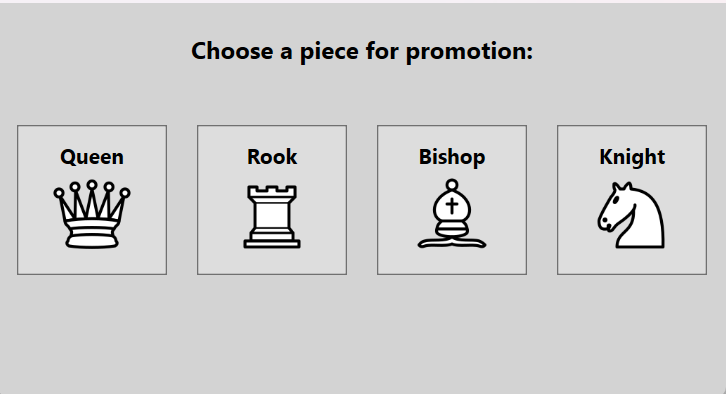
\includegraphics[height=2.3in]{Images/Use Cases/promotionSelectOptions.png}
    \end{center} \\ 
    \hline
\end{longtable}

\subsection{Multi-Player Game Progress}

\begin{longtable}{|m{0.25\textwidth}|m{0.7\textwidth}|}
    \caption{Multi-Player Game Progress} \\
    \hline
    Name & Game page \\
    \hline
    Actor & Player \\
    \hline
    Description & It displays current progress of the game. On top right side are the moves notations, and below are both player's dead pieces\\ 
    \hline
    \centering UI & 
    \begin{center}
        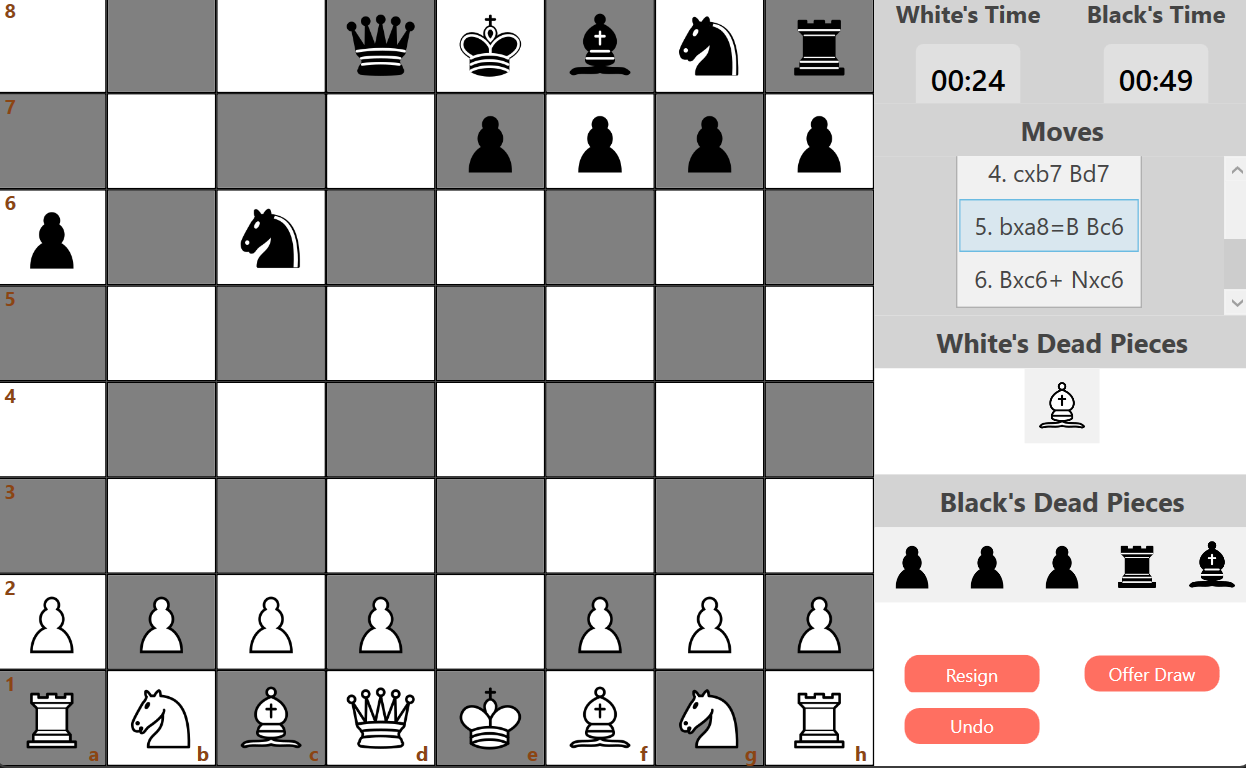
\includegraphics[height=2.7in]{Images/Use Cases/multiplayerProgress.png}
    \end{center} \\ 
    \hline
\end{longtable}

\subsection{Vs Computer Select Options}

\begin{longtable}{|m{0.25\textwidth}|m{0.7\textwidth}|}
    \caption{Vs Computer Select Options} \\
    \hline
    Name & Vs Computer Select Options \\
    \hline
    Actor & Player \\
    \hline
    Description & It displays the time controls, difficulty levels and the color that the player can select.  \\ 
    \hline
    \centering UI & 
    \begin{center}
        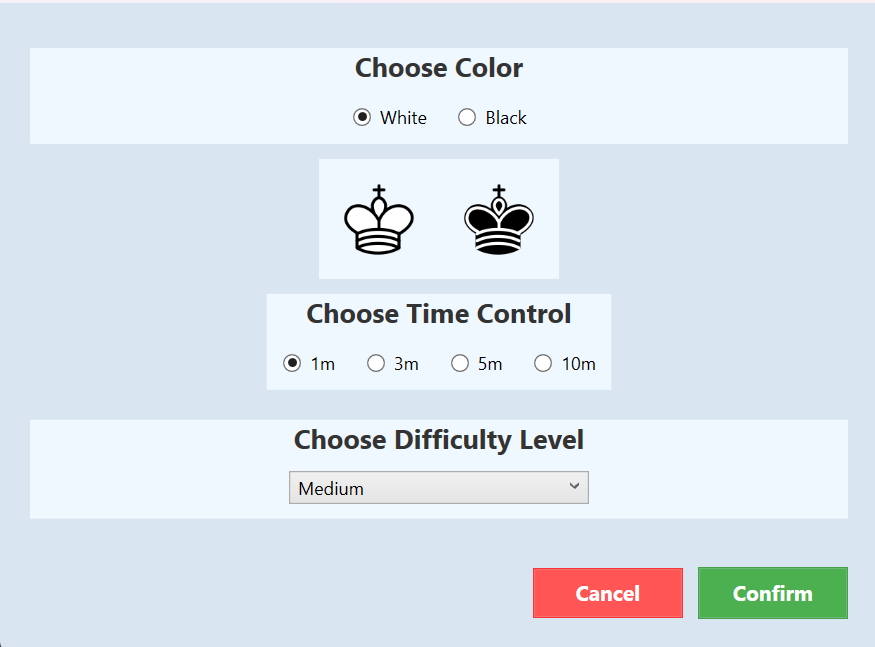
\includegraphics[height=2.7in]{Images/Use Cases/vsComputerSelectOptions.png}
    \end{center} \\ 
    \hline
\end{longtable}

\subsection{Vs Computer Progress Page}

\begin{longtable}{|m{0.25\textwidth}|m{0.7\textwidth}|}
    \caption{Vs Computer Progress Page} \\
    \hline
    Name & Vs Computer Progress page \\
    \hline
    Actor & Player \\
    \hline
    Description & It displays current progress of the game. We can clearly see that the time of Black(Computer) is not used at all which shows it's fast move selection. \\ 
    \hline
    \centering UI & 
    \begin{center}
        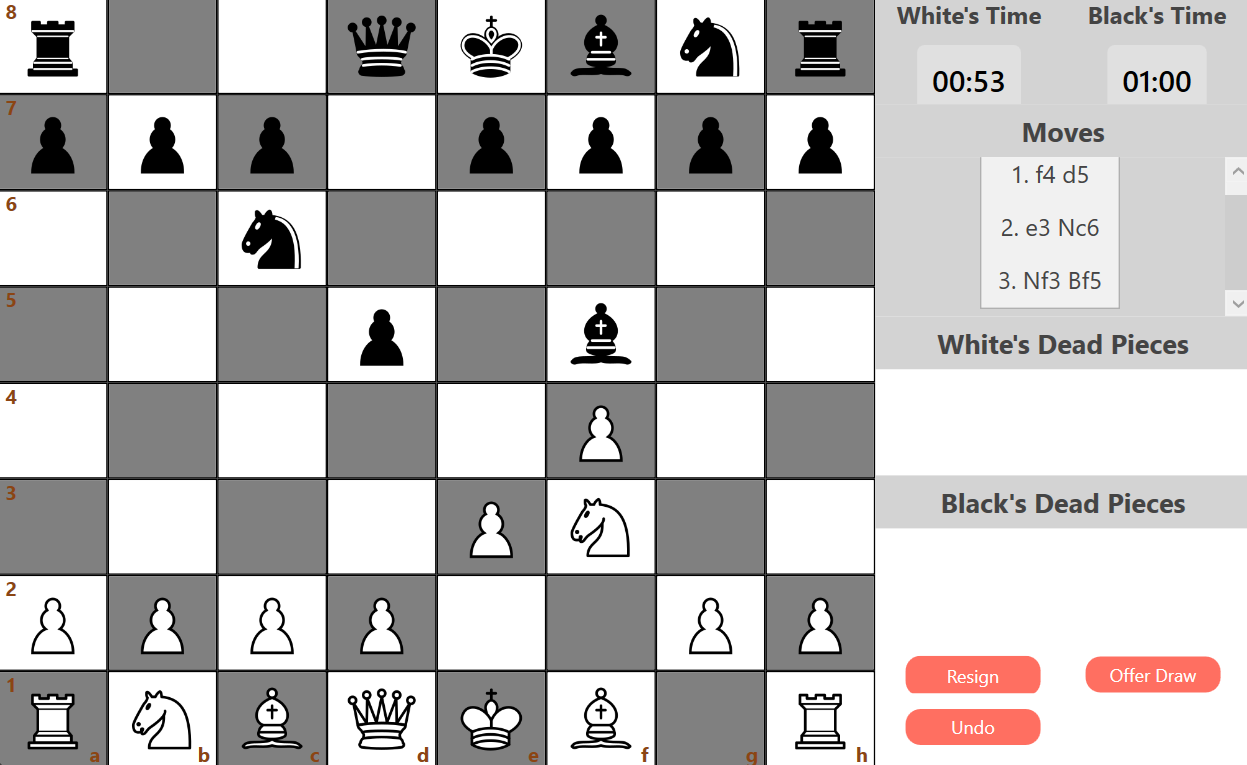
\includegraphics[height=2.7in]{Images/Use Cases/vsComputerProgress.png}
    \end{center} \\ 
    \hline
\end{longtable}

\subsection{About Page}

\begin{longtable}{|m{0.25\textwidth}|m{0.7\textwidth}|}
    \caption{About Page} \\
    \hline
    Name & About page \\
    \hline
    Actor & Player \\
    \hline
    Description & It displays the develepor info, project's features and developer's social links. \\ 
    \hline
    \centering UI & 
    \begin{center}
        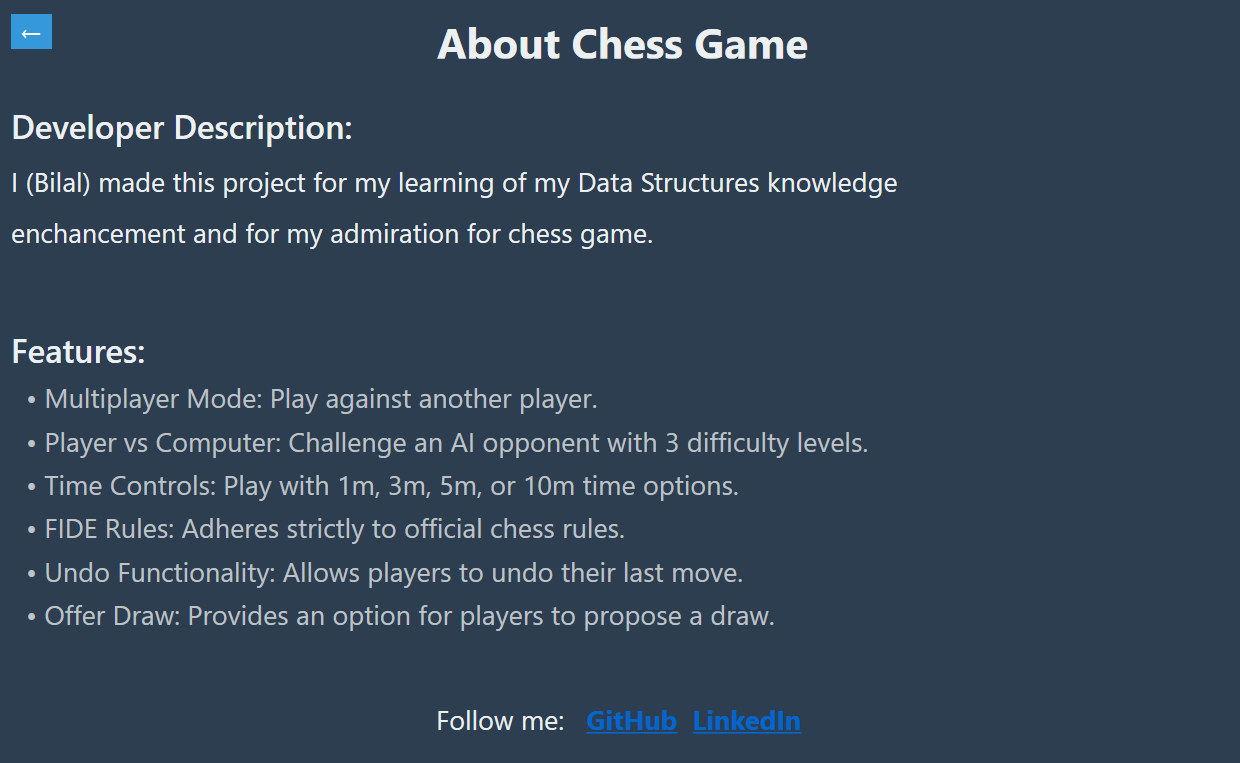
\includegraphics[height=2.7in]{Images/Use Cases/aboutPage.png}
    \end{center} \\ 
    \hline
\end{longtable}

\end{document}
